\documentclass[11pt, titlepage]{article}

\usepackage[margin=1in]{geometry}
\usepackage[strict]{changepage}
\usepackage{float}
\usepackage{fancyhdr}
\usepackage{mhchem}
\usepackage{siunitx}
\usepackage{wrapfig, booktabs}
\usepackage{enumitem}
\usepackage{caption}
\usepackage{commath}
\usepackage{amsmath}
\usepackage[hang]{footmisc}
\usepackage{multicol}
\usepackage{amsfonts}
\usepackage{mathrsfs}
\usepackage{mathtools}
\usepackage{tikz}

% my imports
\usepackage[most]{tcolorbox}
\usepackage{hyperref}
\hypersetup{
    colorlinks,
    citecolor=black,
    filecolor=black,
    linkcolor=black,
    urlcolor=black
}

\newcommand{\experimentDate}{\today}
\newcommand{\className}{CSE 371}
\newcommand{\assignmentname}{Lab 3}
\author{Cameron Jennings (ID: 2029631), Donovan Clay (ID: 2276005)}
\newcommand{\authorLastName}{Jennings, Clay}
\title{\assignmentname}

\date{\parbox{\linewidth}{\centering
\experimentDate
  \endgraf\bigskip
  \className\
}}

\pagestyle{fancy}
\fancyhf{}
\setlength{\headheight}{13.59999pt}
\rhead{\authorLastName\ \thepage}
% \lhead{\experimentShortName}
\lhead{\hyperref[beginning]{\assignmentname}}
\cfoot{\className\ -- \assignmentname}

\usepackage{color}
\usepackage{sectsty}

\definecolor{WordSectionBlue}{RGB}{30, 90, 147}

\allsectionsfont{\color{WordSectionBlue}}

\tcbuselibrary{breakable}


\begin{document}
	\maketitle
 
    \setcounter{tocdepth}{2}
    \begin{center}
        \tableofcontents\label{beginning}
    \end{center}
    \newpage
    
    \section{Design Procedure}
        In this lab, a system is implemented with the ability to play sound through a speaker in the DE1\_SoC. Firstly, there is a module to set up the microphone and speaker. After the initialization process, the microphone begins to read data at a rate of 48,000 times per second to the speaker. The system is also able to be switched from the mic to read a ROM containing a note\ file. Finally, the system has the capability to filter the input to ensure that the output has no additional noise.
    
        \subsection{Task \#1}
            Verilog files are provided with the Audio/Video Configuration and Audio CODEC Interface completed. Once the audio of the DE1\_SoC is initialized, the input from the mic begins to be stored in a 128-element buffer. The purpose of task one is to build a module to pass the notes from the mic buffer to the speaker when the Audio CODEC Interface signals to our circuit that it is ready through the write\_ready and read\_ready signals. Then the two channel data is written to the left or right data wire back to the Audio CODEC Interface to be output by the speaker. \\

            The read and write signals of our circuit to the Audio CODEC Interface are triggered when the read\_ready and write\_ready signals are input. Additionally, the leftdata\_write and rightdata\_write are given leftdata\_read and rightdata\_read respectively.

        \subsection{Task \#2}
            The next step was to create a note file using a Python program in Powershell. With the note file created, a ROM was initialized to hold the data for the corresponding note values. Similar to the previous task, now our module was altered to read the values from the ROM. A counter was implemented to run through the notes in the ROM, looping back at the end, to play a continuous note. Finally, both systems were put together so we could swap between the two tasks using SW[9] on the DE1\_SoC board.
            \begin{center}
                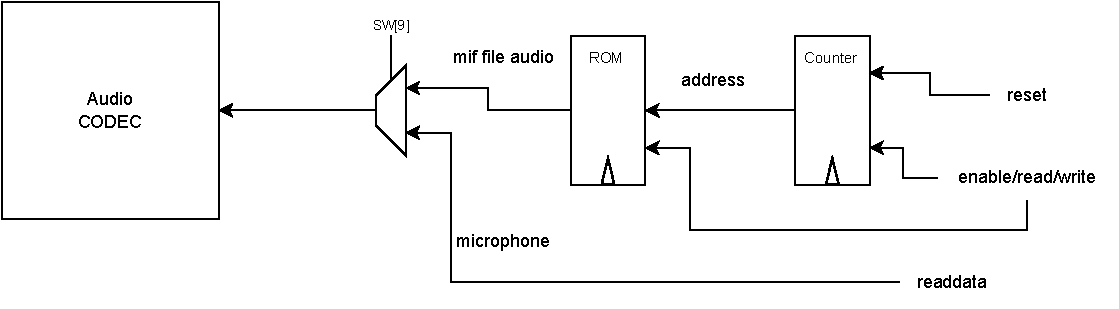
\includegraphics[scale = 0.7]{Images/task 2 block diagram.pdf}
            \end{center}
        
        \subsection{Task \#3}
        The final task in the lab was to create a filter between our circuit and the speaker so that the noise would be eliminated from the either file being played. Given the data from our implemented circuit, the number is scaled to the system and added to a FIFO buffer with a control and datapath. Then the data in the buffer is accumulated into an average of the last N samples so that the transition from data point to data point is smoothed out and the noise is removed from the audio sample. The input to trigger the filter is SW[8].

        The diagram for our filter module is as follows:

        \begin{center}
            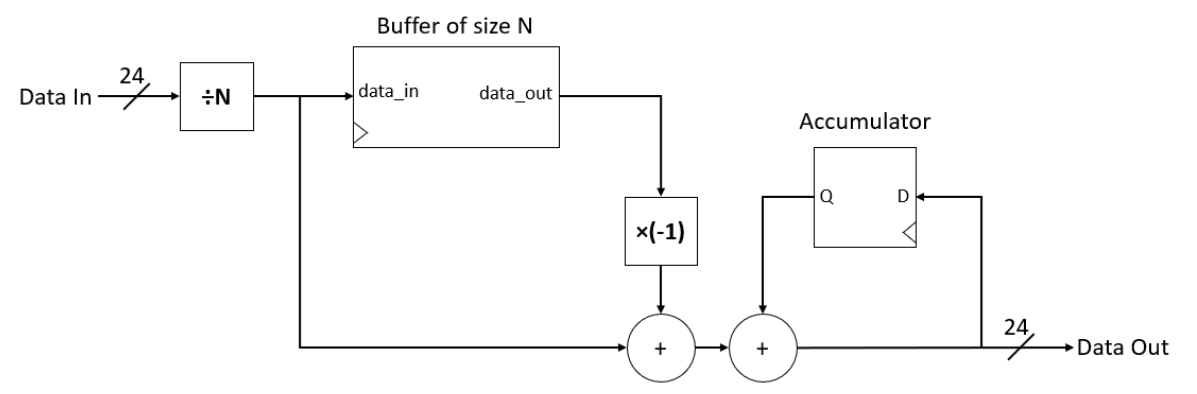
\includegraphics[scale=0.8]{Images/filter diagram.png}
        \end{center}

        \subsection{Task \#3 Overall System Block diagram}
            \begin{center}
                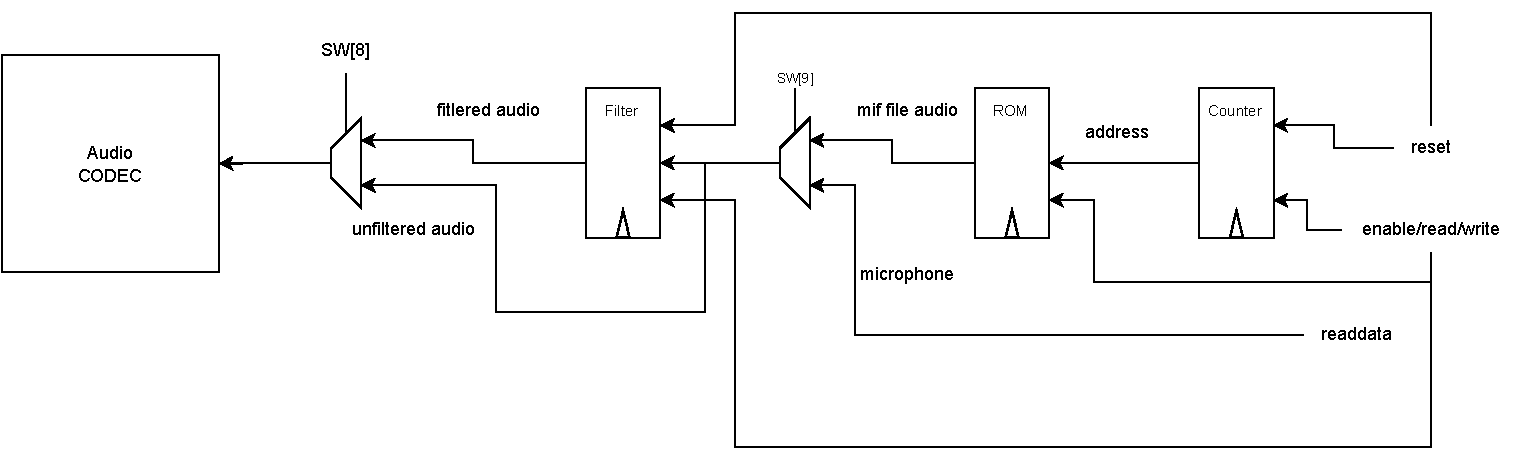
\includegraphics[scale=0.6]{Images/task 3 block diagram.pdf}
            \end{center}
        
    

    \section{Results}
    To reiterate, our system is an audio configuration with the ability to output sounds recorded from either a microphone or a ROM file of notes. It also has the capability to filter the noise it receives from either channel so that outputted sounds are smoothed with less static. The switches on the DE1\_SoC can switch the system to decide which file to read from and whether the filter is on or not.

        \subsection{Task \#2}
            The test bench for the task \#2 can be seen below. \\
            \begin{center}
                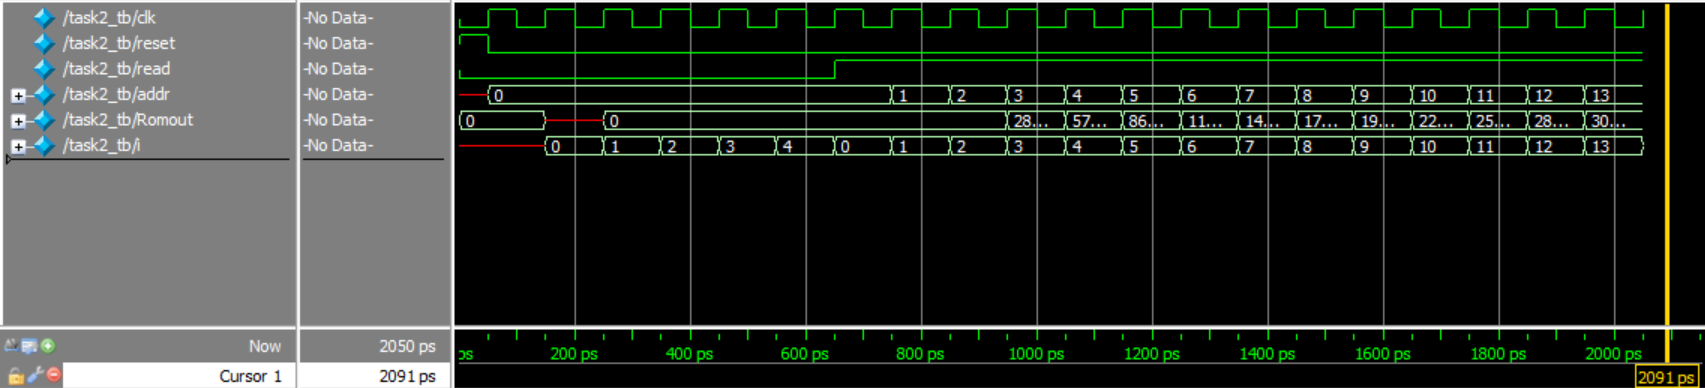
\includegraphics[scale = 0.5]{Images/task 2 testbench.png}
            \end{center}
            This testbench shows that the counter increments when on the positive edge of the clock and when \texttt{read} is asserted. We can also see that the ROM is outputting different data when the read address changes. This demonstrates the expected behavior of the counter and ROM modules.
        
        \subsection{Task \#3}
            The test bench for the task \#3 filter can be seen below. \\
            \begin{center}
                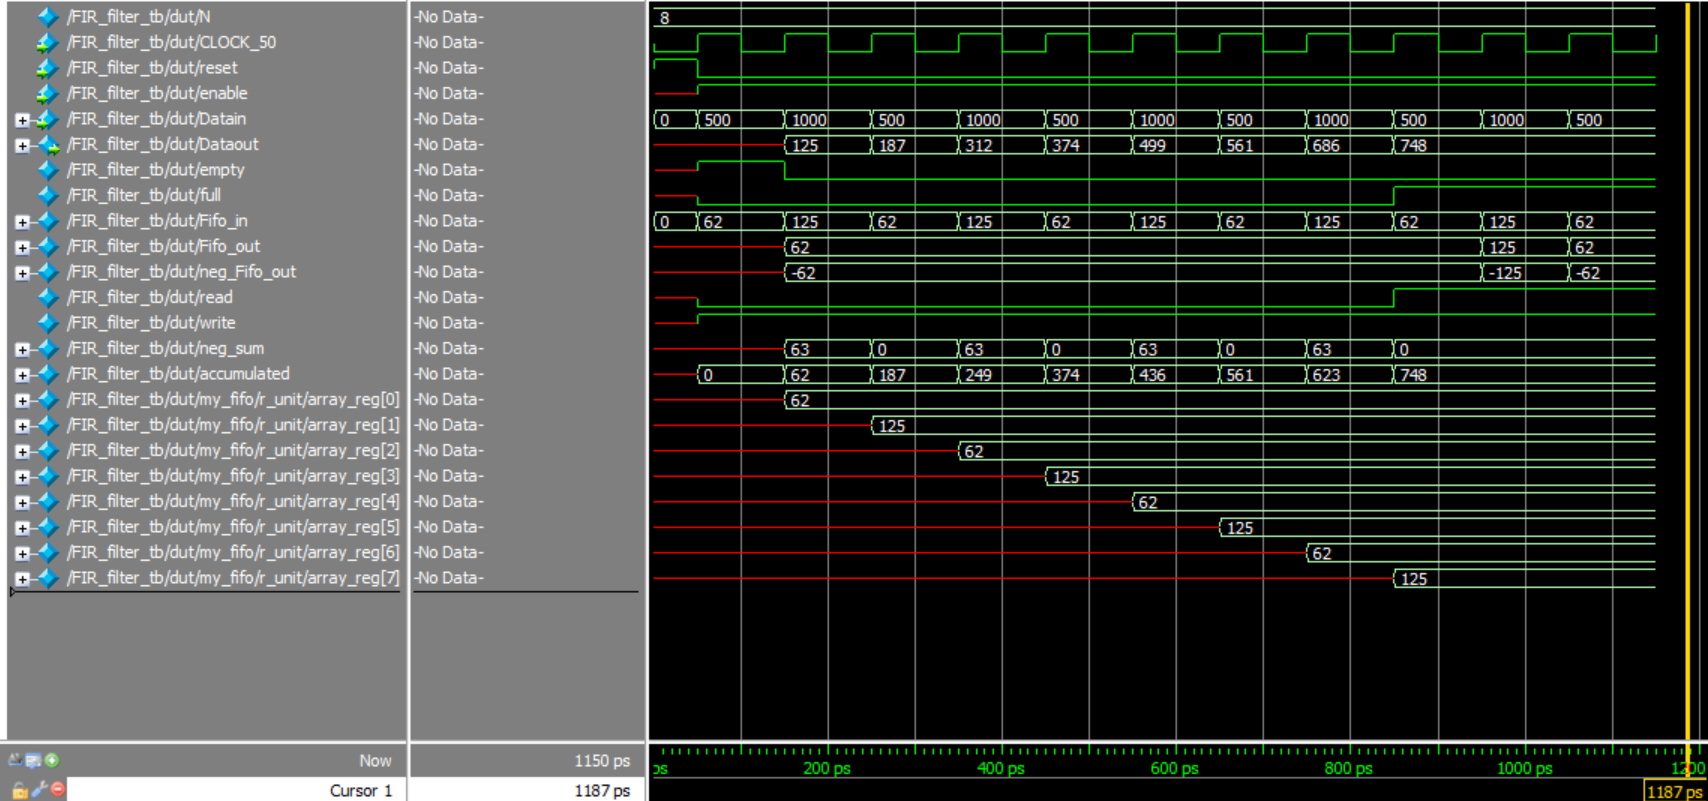
\includegraphics[scale = 0.5]{Images/task 3 filter testbench.png}
            \end{center}
            This testbench shows that the filter correctly takes the average of data that is inputted to it. The testbench alternates between inputting 1000 and 500 to the filter. So we should expect the filter to output about 750 (average of 1000 and 500). We can see that once the buffer in the filter fills up, the filter outputs 748, which is what we want. So this shows the expected behavior.

        \subsection{Flow Summary}
            Fitter Status : Successful - Fri Oct 27 22:35:24 2023 \\
            Quartus Prime Version : 17.1.0 Build 590 10/25/2017 SJ Lite Edition \\
            Revision Name : task2part1\\ 
            Top-level Entity Name : task2part1\\ 
            Family : Cyclone V\\ 
            Device : 5CSEMA5F31C6\\
            Timing Models : Final\\ 
            Logic utilization (in ALMs) : 273 / 32,070 ( $< $1 \% )\\ 
            Total registers : 299\\
            Total pins : 21 / 457 ( 5 \% )\\
            Total virtual pins : 0\\
            Total block memory bits : 1,161,216 / 4,065,280 ( 29 \% )\\
            Total RAM Blocks : 147 / 397 ( 37 \% )\\
            Total DSP Blocks : 0 / 87 ( 0 \% )\\
            Total HSSI RX PCSs : 0\\
            Total HSSI PMA RX Deserializers : 0\\
            Total HSSI TX PCSs : 0\\
            Total HSSI PMA TX Serializers : 0\\
            Total PLLs : 1 / 6 ( 17 \% )\\
            Total DLLs : 0 / 4 ( 0 \% )\\
            
    \section{Experience Report}
        This lab took a while to understand how the starter code worked, but after that it was somewhat straight forward. The filter was similar in the aspect that once we figured out what the specification was saying  and discover some crucial bugs it was not too difficult to implement. Therefore, the debugging and figuring out the starter code were the most difficult parts in this lab.

        A concept that we learned while doing this lab is that we can implement algorithms in hardware. An example of this would be the FIFO buffer or also the filter entirely. The structure of the algorithms can be repurposed for other uses in other labs which is very useful.
    

        This lab took approximately 12 hours, broken down as follows:
        \begin{description}
            \item[Reading:] 45 minutes
            \item[Design:] 15 minutes
            \item[Coding:] 6 hours
            \item[Debugging:] 4 hours
        \end{description}   
        
\end{document}
